\documentclass[12pt]{article}

\usepackage{fullpage}
\usepackage{graphics}
\usepackage{tikz}
\usepackage[parfill]{parskip}
\usepackage[utf8]{inputenc}
\usepackage{etoolbox}
\usepackage{ textcomp }

\newbool{alt}
\booltrue{alt}
%\boolfalse{alt}

% Standard things to include for math
\usepackage{amsmath,amssymb,amsfonts,amsthm}

\usepackage{wasysym}

\usepackage{enumitem}



\usepackage{geometry}
 \geometry{
 a4paper,
 top=3cm,
 bottom=3cm,
 left=2cm,
 right=2cm,
 }




% Some of Ebrahim's definitions
\newcommand{\done}{\\\hspace*{0pt}\hfill$\blacksquare$}
\def\N{\mathbb{N}}
\def\R{\mathbb{R}}
\def\Q{\mathbb{Q}}
\def\Z{\mathbb{Z}}
\def\e{\epsilon}
\newcommand{\seq}[1]{\left(#1\right)_{n\in\N}}
\newcommand{\Euc}[1]{\mathbb{R}^{#1}}
\newcommand{\pathvarNaked}{p}
\newcommand{\pathvar}{\vec{\pathvarNaked}}
\newcommand{\pathvarAlt}{\vec{q}}
\newcommand{\exercisesList}[2]{\textcolor{ForestGreen}{Exercises from WeBWorK HW#1: #2.}}
\newcommand{\exerciseText}[1]{\textcolor{ForestGreen}{Exercise: #1}}
\def\vx{\vec{x}}
\def\vu{\vec{u}}
\def\vv{\vec{v}}
\def\vw{\vec{w}}
\newcommand{\der}[2]{\frac{\textrm{d}#1}{\textrm{d}#2}}
\newcommand{\derOp}[1]{\der{\phantom{#1}}{#1}}
\newcommand{\pder}[2]{\frac{\partial #1}{\partial #2}}
\newcommand{\pderOp}[1]{\pder{\phantom{#1}}{#1}}
\newcommand{\colvectwo}[2]{\left[\begin{array}{c}#1\\#2\end{array}\right]}
\newcommand{\colvectwoXYVEC}[2]{\left[#1\right]\,\cbv{x} + \left[#2\right]\,\cbv{y}}
\newcommand{\colvecthree}[3]{\left[\begin{array}{c}#1\\#2\\#3\end{array}\right]}
\newcommand{\colvecfour}[4]{\left[\begin{array}{c}#1\\#2\\#3\\#4\end{array}\right]}
\newcommand{\colvecfourL}[4]{\left[\begin{array}{l}#1\\#2\\#3\\#4\end{array}\right]}
\newcommand{\norm}[1]{\left|\hspace{-1.5pt}\left|#1\right|\hspace{-1.5pt}\right|}
\def\grad{\vec{\nabla}}
\newcommand{\Dir}[3]{\operatorname{Dir}(#1,#2,#3)}
\newcommand{\D}[1]{\textrm{D}#1}
\def\vn{\vec{n}}
\newcommand{\cbv}[1]{\partial_{#1}}
\newcommand{\arrayBrackets}[2]{\left[ \begin{array}{#1} #2 \end{array} \right] }

\makeatletter
\newcommand*\dotp{\mathpalette\bigcdot@{.5}}
\newcommand*\bigcdot@[2]{\mathbin{\vcenter{\hbox{\scalebox{#2}{$\m@th#1\bullet$}}}}}
\makeatother



\newcommand{\ansbox}[2]{\raisebox{-.5\height}{\framebox(#1,#2){}}}

\def\endans{\hspace{1em}\ansbox{40}{40}}


\newcommand{\NEcheckbox}{ % Put check box on northeast corner of page
\begin{tikzpicture}[remember picture,overlay]
\path (current page.north east) ++(-1,-1) node[below left] {
{\small graded?} {\Large\Square}
};
\end{tikzpicture}
}

\newcommand{\LEFTcheckbox}{ % Put check box in the left margin
\\\begin{tikzpicture}[remember picture,overlay]
\path ++(-2,0) node[below left] {
 {\Large\Square}
};
\end{tikzpicture}
}

\newcommand{\LEFTcheckboxOwnLine}{ % Put check box in the left margin, use this one if on own line
\begin{tikzpicture}[remember picture,overlay]
\path ++(-2,0) node[below left] {
 {\Large\Square}
};
\end{tikzpicture}
}






\pagenumbering{gobble}
\begin{document}




% --- Score table ---

%\def\gap{\hspace*{2.5em}}
%
%\begin{tikzpicture}[overlay, remember picture]
%\path (current page.north east) ++(-1,-1) node[below left] {
%\begin{tabular}{c|c|c|c|c|c|c|c}
% 1 &  2 & 3 & 4 & 5 & 6 & 7 & $\Sigma$\\ \hline
% \gap & \gap & \gap & \gap & \gap & \gap & \gap & \gap \\
% \gap & \gap & \gap & \gap & \gap & \gap & \gap & \gap
%\end{tabular}
%};
%\end{tikzpicture}

% ---


\def\namepos{(current page.north west) ++(5,-0.8)}
\begin{tikzpicture}[overlay, remember picture]
\draw [black] \namepos rectangle ++(10,-1);
\draw [black] \namepos ++(0,-1.2) rectangle ++(10,-1);
%\draw [black] \namepos ++(0,-1.2) ++(0,-1.2) rectangle ++(10,-1);
%\draw [black] \namepos ++(0,-1.2) ++(0,-1.2) ++(0,-1.2) rectangle ++(10,-1);
\path \namepos ++(0,-0.4) node [left] {\textbf{Name:}};
\path \namepos ++(0,-0.4) ++ (0,-1.2) node [left] {\textbf{Perm:}};
%\path \namepos ++(0,-0.4) ++ (0,-1.2) ++ (0,-1.2) node [left] {\textbf{Seat Number:}};
%\path \namepos ++(0,-0.4) ++ (0,-1.2) ++ (0,-1.2) ++ (0,-1.2) node [left] {\textbf{ID Checker Name:}};
\end{tikzpicture}

\def\versionRowText{
\textit{version \ifbool{alt}{1}{2},row}
\raisebox{-3pt}{\framebox(15,15){A}}
}
\begin{tikzpicture}[overlay, remember picture]
\path (current page.north east) ++ (-2,-1.5) node [left]{}; %{\versionRowText};
\end{tikzpicture}



\vspace{5em}

\begin{center}\textbf{Math 34A Final Exam, Summer 2022}

({\it 100 pts total})
\end{center}



\pagebreak

\phantom{.}
%%%%%%%%%%% (1)
\pagebreak
\begin{enumerate}
\item Use the log table provided with this exam to answer the following questions:


\begin{enumerate}
\item Find $\log(3118)$
\vfill
\phantom{.} \hfill$\log(3118) \approx \ $ \ansbox{100}{60}
\item Find $\log(5^{10})$
\vfill
\phantom{.} \hfill$\log(5^{10}) \approx \ $ \ansbox{100}{60}
\item Approximate a solution for $x$ in the equation $$10^{x-5}=5^{10}.$$
(You must use the log table to find a numerical answer.)

\vfill
\vfill
\phantom{.} \hfill$x \approx \ $ \ansbox{100}{60}
%\item Using the approximation in your previous answer as well as the fact that $2^{10}$ is exactly 1024, compare the two values by writing a $<$, $=$ or $>$ in the box below.


%If you are stuck, consider taking the anti-log of both numbers in part (b).
%\vfill
%\phantom{.} \hfill$\log(2) \ $ \ansbox{40}{40} $ \ .3$
\end{enumerate}




\pagebreak
%%%%%%%%%%% (2)
\item ({\it 6 pts}) Find $f'(x)$, where $$f(x)= 2e^{3x} + 3x^2 + 2x + \pi.$$

%\vspace*{1 cm}
\vfill

\hfill $\displaystyle f'(x)=$ \ansbox{300}{70} \vspace{20pt}





%%%%%%%%%%% (5)
\item ({\it 9pts}) Below is the graph of a funtion $g(x)$ with five labeled points, $A$, $B$, $C$, $D$, and $E$. Identify a point where $g''(x) < 0$, a point where $g''(x) = 0$, and a point where $g''(x) > 0$. \vspace{10pt}



%f(x)=0.02 (x+4) (x+2) x (x-2) (x-4) for the graph below in Geogebra
\begin{center}
\fbox{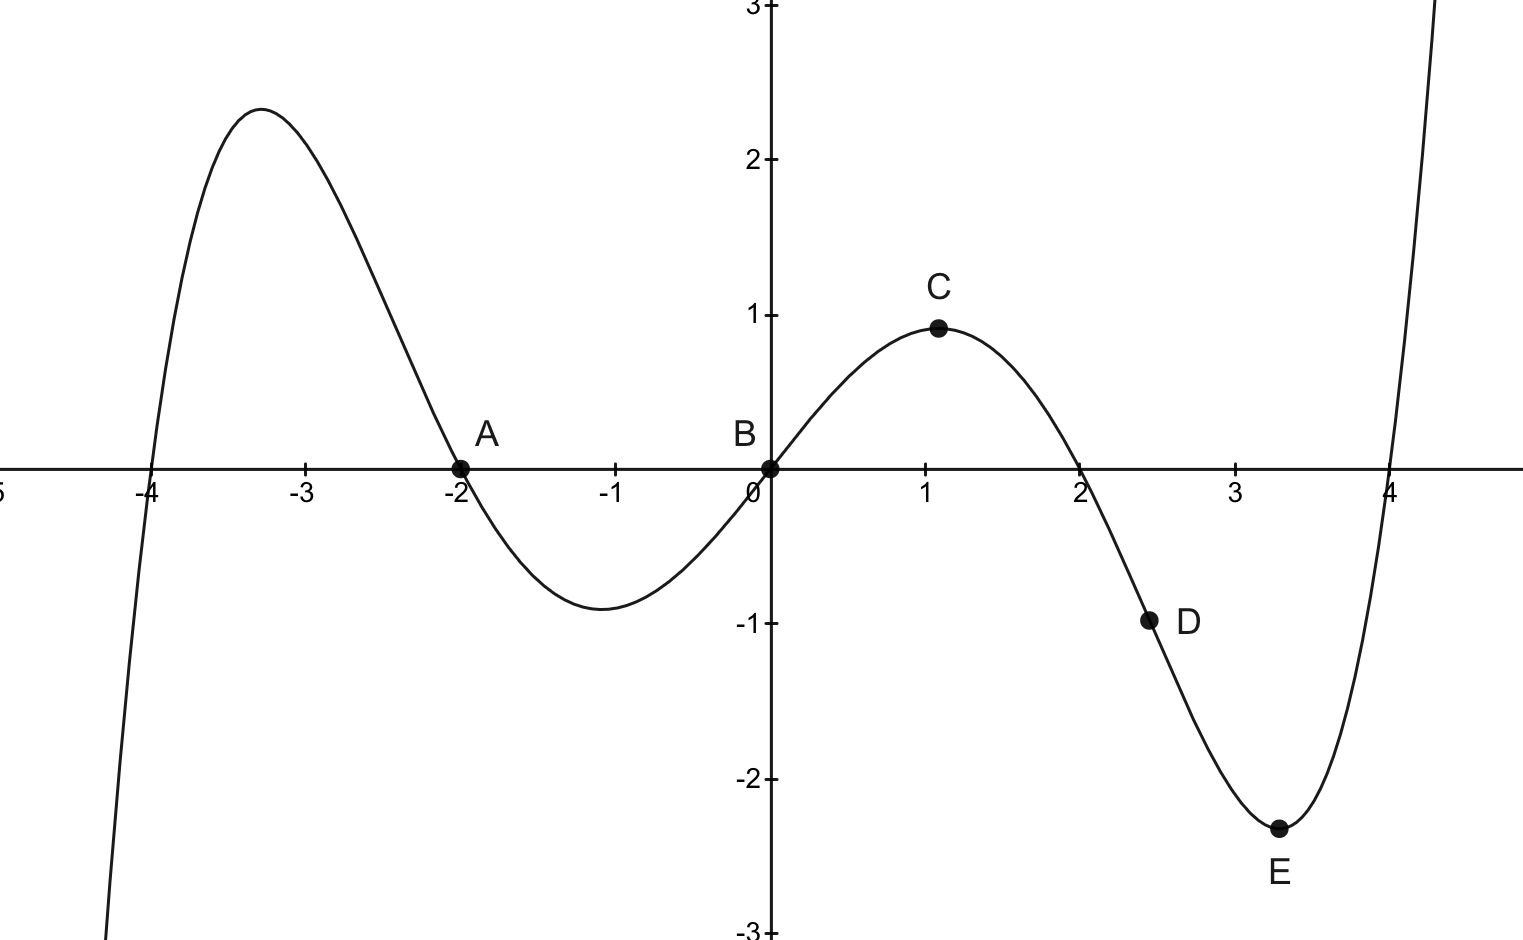
\includegraphics[width=.8\textwidth]{Final_Exam_Graph_Black_ver2}}
\end{center}


\vspace{15pt}


    \phantom{.} \hfill
     \begin{tabular}{rccc}
     \text{Be sure to only write }\textbf{one }\text{point in each box!} & \ansbox{60}{50} \ & \ \ansbox{60}{50} & \ansbox{60}{50} \\
     & $g''(x) < 0$ & $g''(x) = 0$ & $g''(x) > 0$
     \end{tabular}
     \bigskip

\vfill

\pagebreak
%%%%%%%%%%% (3)
\begin{minipage}{.7\linewidth}
\item ({\it 10 pts}) A goblin catapult sits at at the top of a cliff, overlooking the enemy. When it launches, the height of its ``projectile" (see figure) is given by the equation $$f(t)=-5t^2 + 20t + 25,$$ where $t$ is the time in seconds since launch and $f(t)$ is the height (in meters) of the projectile above the enemy. (In this problem we are ignoring horizontal movement.)
\end{minipage} 
\begin{minipage}{.3\linewidth}
%\vspace*{-3ex}
%\hfill
\hspace*{.5 cm}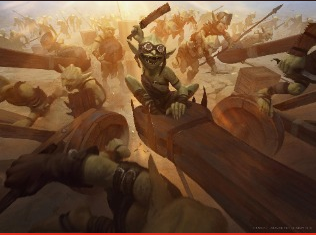
\includegraphics[width=\linewidth]{goblin_cannon}
\end{minipage}

\begin{enumerate}

\item How high is the cliff which the goblin is launched from?

\phantom{.} \hfill \ansbox{100}{50} meters

\item In your own words, interpret $f(1)=40$, $f'(1)=10$. 

\ansbox{\linewidth}{100}

\item What is the goblin's highest altitude?

\phantom{.} \hfill \ansbox{100}{50} meters

\item How long will we be able to hear the projectile cackling maniacally until it strikes the target?

\phantom{.} \hfill \ansbox{100}{50} seconds

\item As time goes by, is the goblin's acceleration increasing, decreasing, or staying the same? Use calculus to justify your response. 

\ansbox{\linewidth}{100}

\end{enumerate}






\pagebreak



%%%%%%%%%%% (6)
\item ({\it 10pts}) For this problem, $f(x) = (x^2+4)(x+3).$ \vspace{20pt}
\begin{enumerate}
\vfill
\item $f'(x)=$\phantom{.} \ansbox{400}{70} \vspace{20pt} %


\vfill
\item $f''(x)=$ \ansbox{400}{70} \vspace{20pt} %


\end{enumerate}




%%%%%%%%%%% (6)
\item ({\it 6pts})  You have 600m of fencing for a rectangular field, but the field needs to also be

\parbox{.5\textwidth}{\vspace*{-30 pt} subdivided into 3 equal areas by fencing as shown in the figure to the right. If $\ell$ and $w$ (length and width) are the dimensions of your pen, the total combined fencing must be 600m, so
    $$4\ell + 2w = 600.$$}
    \parbox{.5\textwidth}{%
      \vspace*{-10 pt}
      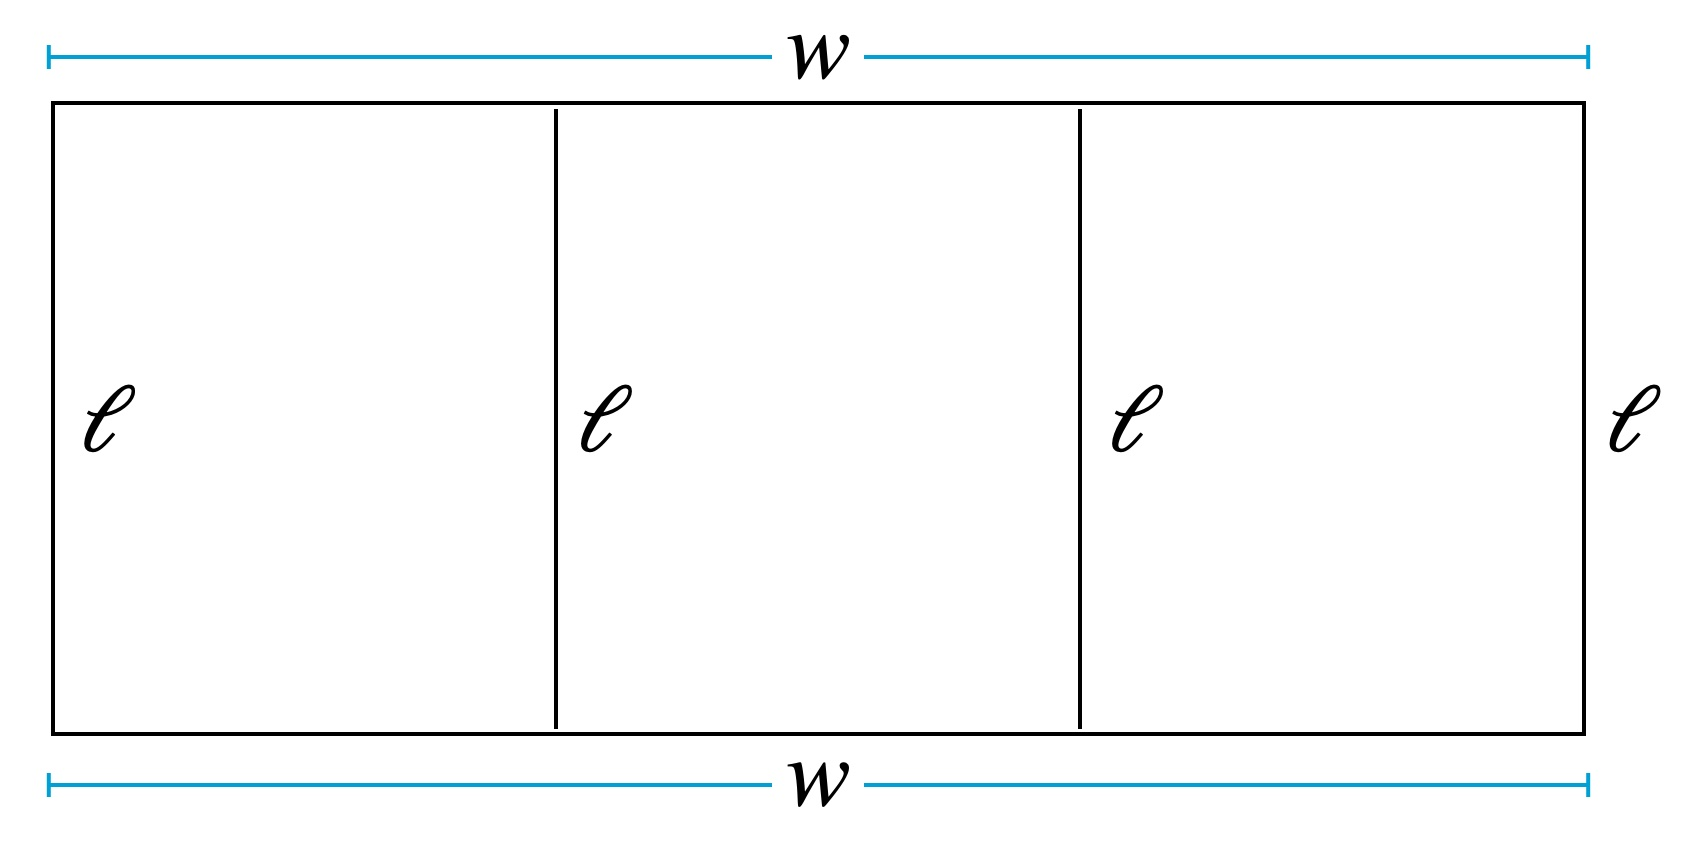
\includegraphics[width=.5\textwidth]{problem_6_figure}
    }

    %Here there are two extra ``lengths'' to serve as dividers between the three subdivisions.

    \begin{enumerate}
    \item %You know the area of the pen in terms of $\ell$ and $w$.
    Express the \textbf{area} of the pen in terms of \underline{$\ell$ only}. \vfill

    \hfill$A(\ell) =$\ \ansbox{190}{50} \phantom{i} m$^2$
    \item Find the length that results in the largest area $A(\ell)$ for your field. \vfill

    \hfill$\ell =$\ \ansbox{190}{50} \phantom{i} m\phantom{$^2$}
    \item Use your answer in part (b) to find the maximum area for your field. \vfill

    \hfill $A_{\text{max}} =$\ \ansbox{190}{50} \phantom{i} m$^2$
    \end{enumerate}

    \pagebreak





\pagebreak
%%%%%%%%%%% (7)
\item ({\it 15pts}) Jack Johnson* will be playing at the Santa Barbara Bowl next fall. He gives you 100 concert tickets, asking you to sell them on campus for a charity and to give away any left-over tickets. The price is up to you, but you need to sell them all at the same price. If the price you set is \$20 each then you would sell all 100 tickets. For each dollar you decide to increase the price, the number of tickets you could sell would decrease by 2.
\begin{enumerate}
\item If your ticket price is
$\$x$, how many tickets would you be able to sell?


\vspace{30pt}


\phantom{.} \hfill  \ansbox{150}{50} tickets
\item What is the total revenue (in terms of $x$) you would receive for selling those tickets? You do not need to simplify your answer for this part.


\vfill
\phantom{.} \hfill { \$} \ \ansbox{350}{50}
\item What is the optimal ticket price, and how much money would you raise for charity altogether at that price?


\vfill
\vfill
\vfill
\phantom{.} \hfill { price: \$} \ \ansbox{80}{50} { maximum revenue: \$} \ \ansbox{80}{50}
\end{enumerate}
\scriptsize{*Maybe this story isn't so far-fetched. Jack Johnson is a UCSB alumnus and after he heard about a tragic event that happened here a few years ago he came and played a free concert in front of Storke Tower. He also fund-raises frequently for people in need in this area, including a benefit a couple months ago for victims of the Thomas fire.}


%    \pagebreak
%    \phantom{.}













\end{enumerate}



\end{document}
